% !TeX root = RJwrapper.tex
\title {Unified ROC Curve Estimator for Diagnosis and Prognosis Studies: The sMSROC Package}
\author{\phantom b\par\noindent by Susana D\'iaz-Coto, Pablo Mart\'inez-Camblor and Norberto Octavio Corral-Blanco}

\maketitle

\abstract{
The binary classification problem is a hot topic in Statistics. Its close relationship with the diagnosis and the prognosis of diseases makes it crucial in biomedical research. In this context, it is important to identify biomarkers that may help to classify individuals into different classes, for example, diseased vs. not diseased. The Receiver Operating-Characteristic (ROC) curve is a graphical tool commonly used to assess the accuracy of such classification. Given the diverse nature of diagnosis and prognosis problems, the ROC curve estimation has been tackled from separate perspectives in each setting. The Two-stages Mixed-Subjects (sMS) ROC curve estimator fits both scenarios. Besides, it can handle data with missing or incomplete outcome values. This paper introduces the \url{R} package sMSROC which implements the sMS ROC estimator, and includes tools that may support researchers in their decision making. Its practical application is illustrated on three real-world datasets.}

\section{Introduction} \label{sec:s1}
The binary classification problem is crucial in biomedical environments. Researchers and physicians face the task of classifying patients (as e.g. diseased vs. disease-free, at risk vs. risk-free, etc.) daily. Frequently, biological measures (biomarkers) are used as objective medical signs that may indicate, for example, the presence/progress of an event of interest or the response to specific treatments.
Diagnostic biomarkers are normally employed to detect the presence of a disease. For example, the \textit{circulating cardiac troponin I} aids in noninvasive detection of myocardial injury in cardiovascular diseases \citep{Ni2018}. The \textit{blood glucose} and the \textit{hemoglobin A1c} are recognized diagnostic biomarkers of type 2 diabetes mellitus \citep{Long2020} and the \textit{sweat chloride} is often used to confirm the cystic fibrosis \citep{Farrel2008}.

The Receiver Operating-Characteristic (ROC) curve is a popular graphical tool for assessing the ability of biomarkers to discriminate between positive and negative individuals (with and without the event of interest, respectively)  \citep{Zhou2002, Pepe2003}. For each possible cut-off point, it plots the pairs formed by the complement of {\it specificity} against the {\it  sensitivity}. The sensitivity, {\it {Se}}, and the specificity, {\it {Sp}}, are the proportions of positive and negative individuals, respectively, who have been correctly classified.
The closer the ROC curve to the upper left corner, the more accurate the biomarker.

Mathematically, for each $u\in [0,1]$, the ROC curve has the expression:
\begin{equation}
{\cal R}(u)= Se\left(Sp^{-1}(1-u)\right), \label{R11}
\end{equation}
where $Sp^{-1}(\cdot) = \inf \{x: Sp(x) \geq \cdot\} $. Conventionally, it is assumed that individuals with larger biomarker values are more likely positive. Therefore, the classification sets defining an individual as positive are those in the way $[c, \infty)$, with  $c = Sp^{-1}(1-u) \in\mathbb{R} $. Besides, the related area under the ROC curve, (AUC) $\left(=\int_{0}^{1}{{\cal R}(u)du}\right)$, is commonly used as a summary index of the global classification accuracy \citep{hanl82}. 

The estimation of ROC curves has been addressed from different perspectives (see, for instance, \citet{gon14} and references therein). Estimation procedures generally assume that data come from case-control designs, where the actual status of all individuals as positive or negative is known in advance. Further, they do not handle the issue of potential missing values in the outcome. Notice that such issues arise, for instance, in cohort designs where the outcome is defined ad hoc through a subsidiary variable. The missing values for that variable lead to missing values in the outcome.

Most of the statistical software (SPSS, SAS, STATA, etc.) offer routines for computing different ROC curve estimators and related elements. There are also packages in \url{R} (\url{www.r-project.org}) dealing with the ROC curve topic. We highlight the \CRANpkg{pROC} package \citep{robin11},  which provides functions for visualizing, smoothing and comparing ROC curves; the package \CRANpkg{nsROC} \citep{nsROC}, where some of the non-standard tools for the ROC curve analyses described in \citet{Perez-Fernandez2018}  are implemented; the package \CRANpkg{ROCR} \citep{ROCR}, which supplies user-friendly tools for creating graphics for visualizing classification performance (the ROC curve is a particular case); the \CRANpkg{plotROC} package \citep{Sachs2017}, offering interactive ROC curve plots suitable for use on the web, and finally the \CRANpkg{ROCnReg} package \citep{Cote2021}, which, among other extensive functionality, implements Bayesian methods for the estimation of ROC curves.

Prognostic biomarkers are used to identify individuals who are likely to experience a future clinical event (death, the onset/recurrence of a disease or the development of a new medical condition). For example, the breast cancer genes 1 and 2 mutations are often employed to assess the likelihood of a second breast cancer \citep{Basu2015}. Similarly, the C-reactive protein level is a prognostic biomarker used to identify individuals with unstable angina at risk of developing other adverse events \citep{Ferreiros1999}, and the Gleason score helps to assess the likelihood of prostate cancer progression \citep{Epstein2016}. These biomarkers are measured at baseline and individuals are then followed over time to observe whether or not the event of interest occurs. 
A {\it{time-to-event}} variable is involved in this process. Different definitions of positive and negative outcomes have been proposed, which has given rise to extensions of the sensitivity and specificity measures and, of course, to the corresponding time-dependent ROC curves \citep{Etzioni99} .

The Cumulative/Dynamic (C/D) ROC curve \citep{Heagerty2000} is perhaps the most natural extension of the ROC curve for time-dependent outcomes. Once set to a specific point of time $t$, the time-to-event variable is reduced to a dichotomous variable at that time. Then, the sensitivity and the specificity can be extended to the so-called {\it {cumulative sensitivity }} and {\it{dynamic specificity}} whose expressions are 
\begin{equation*}
Se_{t}^{\mathbb{C}}(c) = {\cal{P}}(X > c \;| \; T \leq t),
\end{equation*}
\begin{equation*}
Sp_{t}^{\mathbb{D}}(c) = {\cal{P}}(X \leq c \;| \; T > t),
\end{equation*}
where $c \in \mathbb{R}$ is the cut-off point, and $X$ and $T$ are the random variables modeling the biomarker and the time-to-event variables, respectively. The C/D ROC curve is the plot of the pairs formed by the complement to the dynamic specificity and the cumulative sensitivity, for all possible cut-off points. Alternatively, it is given by
\begin{equation*}
{\cal R}_{t}^{{\mathbb{C}}/{\mathbb{D}}}(u)= Se_{t}^{\mathbb{C}}\left([Sp_{t}^{\mathbb{D}}]^{-1}(1-u)\right), \quad u \in[0,1].	
\end{equation*}
The area under the C/D ROC curve is used as well as a summarize index of the prognostic accuracy of a biomarker and has the expression
\begin{equation*}
{AUC}_{t}^{\mathbb{C}/\mathbb{D}} = \int_{0}^{1}{{\cal R}_{t}^{{\mathbb{C}}/{\mathbb{D}}}(u)du}.
\end{equation*}

The main challenge when estimating the C/D ROC curve is the potential lack of complete information for some individuals (caused by censoring). It arises because of loss of follow-up, either due to dropouts or because the study ended before the event of interest had the chance to occur in the individual (right censoring). It may also come up when individuals are not constantly monitored and the only available information is that the event of interest occurred between two observed timepoints (interval censorship). The simplest C/D ROC curve estimator removes from the sample the censored observations and approximates the cumulative sensitivity and the dynamic specificity through their empirical estimators (naive method). Other procedures integrate, in some way, the information from the censored observations.  \citet{Kamarudin2017} provides an illustrative revision of the available \url{ R} packages implementing some of these methods, all of them addressing the right censorship problem. For example, the \CRANpkg{survivalROC} package \citep{survivalROC} computes the C/D ROC curve through the two procedures proposed by \citet{Heagerty2000}. The \CRANpkg{survAUC} package \citep{survAUC} collects several routines for computing the AUC$_{t}^{\mathbb{C}/\mathbb{D}}$, at different times, estimated by the Inverse Probability Censoring Weighting (IPCW) method \citep{Uno2007, Hung2010} and by the \citet{Chambles2006} approach. The \CRANpkg{timeROC}  package \citep{timeROC} implements the Conditional Inverse Probability Censoring Weighting (CIPCW) procedure \citep{Blanche2013}. In addition to confidence intervals for the AUC$_{t}^{\mathbb{C}/\mathbb{D}}$, the package performs tests for comparing two areas under the curve corresponding to different prognostic biomarkers. We add to this list the already mentioned \CRANpkg{nsROC} package, which allows to compute the estimation procedures proposed in \citet{Martinez-Camblor2016} and \citet{li18}. The latter method is also available in the \CRANpkg{tdROC} package \citep{tdROC}. Finally,  the \CRANpkg {smoothROCtime} \citep{Diaz-Coto2020a} and \CRANpkg{cenROC}  \citep{cenROC} packages implement the smooth C/D ROC curve estimators suggested by \citet{Martinez-Camblor2018} and \citet{Kassu2020}, respectively. We only found two packages implementing the C/D ROC curve estimation under interval censorship. The \CRANpkg{intcensROC} package \citep{intcensROC} computes the estimator for the C/D ROC curve and AUC$_{t}^{\mathbb{C}/\mathbb{D}}$ proposed in \citet{Wu2020}, while the \CRANpkg{cenROC} implements the method proposed in \citet{Kassu2022}. Not a package but an \url{R} function is provided in  \citet{Diaz-Coto2020}, computing the C/D ROC curve estimator proposed in that paper.

We present here the package \CRANpkg{sMSROC}, which implements the so-called Two-stage Mixed-Subjects (sMS) estimator. The sMS estimator uses, in a first stage, a probabilistic model for linking the biomarker with the outcome, and then, in a second stage and for each potential threshold, it computes both the sensitivity and the specificity values, which can be used to draw the ROC curve. This approach can be used to answer both diagnostic and prognostic questions, and, by imposing additional constraints on the missing-value mechanism, is able to handle missing data in the outcome variable. The probabilistic model is used for allocating subjects into the positive and the negative groups with certain probabilities. In this sense, subjects are simultaneously classified as positive and negative, that is, they are mixed. Interested readers are referred to  \citet{Diaz-Coto2021} for a more in depth explanation of the theoretical properties of the sMS estimator. The presented \CRANpkg{sMSROC} package offers a set of exploratory tools which help to choose the most suitable probabilistic model (logistic regression, proportional hazard Cox regression, etc.). These (more standard) estimation proposals are already implemented in the package, which also allows to manually enter any other estimates of the probabilities of being positive or negative, which may be estimated by other methods. Among other functionalities, the \CRANpkg{sMSROC} package computes the AUC with confidence intervals, and provides plots for the ROC curve estimates, the predictive models, and the evolution of the AUCs across the follow-up time, providing different options for customizing the final graphics.

The remainder of the  paper is organized as follows. In the Section 2, we present the sMS estimator and review its main properties. We provide a general insight of the structure of the  \CRANpkg{sMSROC} package in the Section 3. In Section 4 the main functions are described in detail. Two real-world datasets are used to illustrate the use of these functions in the diagnosis and prognosis scenarios. In the Section 5, we present a third real-world example, and show how the package can be used to assess the prognostic ability of a biomarker when data are interval censored. We want to present a disclaimer that the examples that the analyses provided here are used to demonstrate the use of the package only and they should not be used to inform any clinical decisions. Finally, we end in the Section 6 with a discussion of the potential uses of the sMSROC package.

\section{The two-stage mixed subjects receiver operating-characteristic curve estimator} \label{sec:s2}
We first introduce the notation that will be used along this paper. Let $X$ be a continuous random variable, with Cumulative Distribution Function (CDF) $H(\cdot)$, which models the behavior of the biomarker values. Let $D$ be the binary random variable representing the event of interest, taking, without lost of generality, values $0$ and $1$, identifying negative and positive individuals, respectively. For prognosis scenarios, let $T$ be the involved time-to-event random variable and let our aim be to predict the occurrence of the event of interest before a fixed point of time $t$. The binary variable depicting this event is given by $D_{t}$, which again takes the values $0$, when $T >t$ (negative individuals) and $1$, when $T \leq t$ (positive individuals). For sake of simplicity, we will remove the subscript $t$ and will use the same notation in both scenarios. 

The expression of the sensitivity can be written as
\begin{align}
 Se(c)  =& {\mathcal P}(X>c\,|\,D) \nonumber\\
          =& \frac{{\mathcal P}(X>c,\,D)}{{\mathcal P}(D)} \nonumber\\
          =&\frac{\mathbb E_X[{\mathcal P}(X>c,\,D\,|\,X =x)]}{\mathbb E_X[{\mathcal P}(D\,|\, X = x)]}\nonumber \\
         =&\frac{\mathbb E_X[{\mathbb {I}}_{(c,\infty)}(x)\cdot {\mathcal P}(D\,|\,x)]}{\mathbb E_X[{\mathcal P}(D\,|\, x)]}\nonumber \\
          =&\frac{ {\displaystyle \int }[{\mathbb {I}}_{(c,\infty)}(x)\cdot {\mathcal P}(D\,|\,x)]dH(x)}{{\displaystyle \int }({\mathcal P}(D\,|\, x))dH(x)}, \label{R21}
\end{align}
where $c \in \mathbb{R}$; ${\mathbb {I}}_A(x)$ depicts the indicator function; $D$ stands for the positive outcome ($D = 1$), and ${\mathcal{P}}(D\,|\,x) = {\mathcal{P}}(D\,|\,X =x) $. 

Similarly, the specificity has the expression:
\begin{align}
Sp(c)  =& {\mathcal P}(X \leq c\,|\,\overline{D}) \nonumber\\
          =& \frac{{\mathcal P}(X \leq c,\,\overline{D})}{{\mathcal P}(\overline{D})} \nonumber\\
          =&\frac{\mathbb E_X[{\mathcal P}(X  \leq c,\,\overline{D}\,|\,X=x)]}{\mathbb E_X[{\mathcal P}(\overline{D}\,|\, X=x)]}\nonumber \\
          =&\frac{\mathbb E_X[{\mathbb {I}}_{(-\infty,c]}(x)\cdot ( 1 - {\mathcal P}(D\,|\,x))]}{\mathbb E_X[{( 1 - \mathcal P}(D\,|\, x))]}\nonumber \\
          =&\frac{{\displaystyle \int } [{\mathbb {I}}_{(-\infty, c]}(x)\cdot(1- {\mathcal P}(D\,|\,x))]dH(x)}{{\displaystyle \int }(1 - {\mathcal P}(D\,|\, x))dH(x)}, \label{R22}
\end{align}
where $\overline{D}$ depicts the negative outcome ($D = 0$).

Let $({\mathcal{X}}_N, {\mathcal{D}}_N) = \{(x_1, d_1), \cdots, (x_N, d_N)\}$ be an independent random sample where, for the $i$-th individual $(1 \leq i \leq N)$, $x_i$ is the biomarker value and $d_i$ reports some information regarding the outcome of interest. Such information, in the diagnosis scenario, may provide the actual status of the individual ($d_i = \delta _i$, where $\delta_i = 0$ for a negative individual, or $\delta_i = 1$, for a positive one) or may be missing. When dealing with a time-dependent outcome, this information can also include the event/censoring time, according to the censorship pattern. That is, in the case of right censorship, $d_i =  \{\delta_i, z_i\}$, being $z_i = \min\{t_i, c_i\}$, where $t_i$ and $c_i$ stand for the event and censoring times, respectively. Under interval censorship, $d_i = \{l_i, r_i\}$, where $l_i$ and $r_i$ are the lower and upper bounds of the observed interval containing the event time $(l_i \leq t_i \leq r_i)$. 
The sensitivity and specificity given in (\ref{R21}) and (\ref{R22}) can be estimated through:
\begin{align}
{\widehat{Se}}(c) = & \frac{{\displaystyle \sum}_{i=1}^N I_{(c,\infty)}(x_i)\cdot {\widehat{\mathcal{P}}_N}(D\,|\,x_i)}{{\displaystyle \sum}_{i=1}^N{\widehat{\mathcal{P}}_N}(D\,|\,x_i)}, \label{R23}\\
{\widehat{Sp}}(c) = & \frac{{\displaystyle \sum}_{i=1}^N I_{(-\infty,c]}(x_i)\cdot (1 - {\widehat{\mathcal{P}}_N}(D\,|\,x_i))}{{\displaystyle \sum}_{i=1}^N(1 - {\widehat{\mathcal{P}}_N}(D\,|\,x_i))}, \label{R24} \quad c \in \mathbb{R},
\end{align}
where ${\widehat{\mathcal{P}}_N}(D\,|\,x)$ is chosen to be an adequate estimator of ${\mathcal{P}}(D\,|\,x)$. 

Plugging-in the expressions (\ref{R23}) and (\ref{R24})  in the definition of the ROC curve given in (\ref{R11}), we obtain the \textbf{Two-stage Mixed Subject (sMS) ROC curve estimator}, to which we will refer as sMS estimator:
\begin{equation*}
{\widehat{\mathcal{R}}}(u) = {\widehat{Se}}\left( [1 - {\widehat{Sp}}]^{-1} (u) \right), \quad u \in [0,1], \label{R25}
\end{equation*}
where  ${\widehat{Sp}}^{-1}(\cdot) = \inf  \{x:{\widehat{Sp}}(x) \geq \cdot \}$.

We briefly review some features of the sMS estimator already introduced in \citet{Diaz-Coto2021}:
\begin {itemize}

\item{The relationship between the biomaker and the outcome is modeled by $\mathcal{P}(D\,|\,x)$ (the predictive model). In the first stage, the sMS estimator approximates the predictive model through the most suitable probabilistic model (e.g. proportional hazards, logistic regression). In the second stage, the rest of the unknown parameters is estimated by the corresponding empirical estimators. The first stage is specially important because the performance of the sMS estimator is highly dependent on the fit of the predictive model to the actual relationship between the biomarker and the outcome.}

\item{The sMS estimator does not need to consider the individuals as fully positive or fully negative. Each individual can be modeled as mixed: partially positive and partially negative (hence the name ``mixed subjects''). The weight allocated to each possibility is determined by the predictive model considering the biomarker value in the specific individual.}

\item{The sMS estimator can handle missing values in the outcome as well as censored observations (latter frequently associated with prognosis studies). The individuals with missing outcome are supposed to be missing at random (MAR) however; that is, their characteristics in the sample should be similar to those with complete information. Under this assumption, their potential outcome is determined by the predictive model for the particular biomarker value.}

\item{The sMS estimator generalizes some of the ROC and C/D ROC curve existing estimators. In the simplest diagnosis scenario, where the real status of all individuals is known, we can estimate the predictive model  $\mathcal{P}(D\,|\,x)$  through the average of the status of those having a biomarker value of $x$. The resulting estimator would be the well-known empirical ROC curve estimator \citep{Hsieh1996}. In the prognosis scenario, considering the adequate estimators for the predictive model, it is clear the connection with the C/D ROC curve estimators under right censorship proposed in \citet{Martinez-Camblor2016} and \citet{li18}, and with the estimator proposed in \citet{Diaz-Coto2020} under interval censorship.  For particular parametrizations, the sMS estimator can as well be the C/D ROC curve estimator proposed  by \citet{Chambles2006} and by \citet{Song2008}.}

\item{Under certain conditions both the sMS estimator and its corresponding estimator for the AUC are asymptotically normal distributed. We provide two approximations for the variance of the AUC estimator: the Theoretical Variance Estimation (TVE), based on a theoretical expression, and the Empirical Variance Estimator (EVE), which avoids dealing with the expression of the variance of the predictive model. Explicit expressions for both the TVE and the EVE approximations are provided in the Appendix of this manuscript. Reported confidence intervals are ${\cal A}\pm\lambda_{\alpha}\cdot\hat \sigma$, with ${\cal A}$ and $\hat\sigma^2$ the AUC and variance approximations, respectively, and $\lambda_\alpha$ the adequate quantile based on the normal distribution.}
\end{itemize}

It is worth clarifying that, although related, the sMS estimator is not a single imputation procedure. In this sense, we are not considering here the presence of missing data in the biomarker. The goal of the sMS estimator is not to impute the unknown values of the outcome, but to use the estimated probabilities to approximate the ROC curve. These probabilities could be used even for those subjects for whom we already know the actual status. For instance, in a standard study in which we collect the status of each single participant, the empirical model would be an extreme situation in which the probability of being positive is determined by the actual observed status of the subject (probability $1$ or $0$). As we have already noted, in this case, the resulting sMS estimator would be the empirical ROC curve estimator. However, we could model these probabilities by the standard binary logistic regression to obtain a smoothed ROC curve estimate. For sure, the quality of this estimation would depend on the goodness of fit of the regression model. For time-to-event outcomes, we can use the actually observed follow-up times for computing the probabilities. Notice that, if the target of interest is to predict events prior to the point $t=5$, participants who still alive at point $4.99$ are more likely to be alive at $5$ than those censored at $0.01$. One of the main advantage of the sMS estimator is its flexibility, which allows to adapt the procedure to several types of data, including different censoring models, and provides a variety of techniques under the same umbrella.

\section{An overview of the package}
The main goal of the \CRANpkg{sMSROC} package (available at \url{https://CRAN.R-project.org/package=sMSROC}) 
is to compute the sMS estimator and related elements, which support the assessment of the diagnostic/prognostic ability of continuous biomarkers. Since \texttt{R} programming is mostly based on objects \citep{Monica2014}, the \CRANpkg{sMSROC} package consists in a set of functions performing specific tasks.

Table \ref{T1}  provides a summary of these functions, grouped by their common features. The functions have been classified as primary and secondary. Among the former, we consider those directly run by the end-user to perform the exploratory data analysis, compute the sMS estimator and other metrics (such as the AUC and its confidence interval), and to summarize the computed results. We refer to the rest of the functions as secondary, as these are mainly called by other functions and not meant to be used by the end-user, primarily. We will describe the primary functions in more detail in the next sections.

The \CRANpkg{sMSROC}  package uses some functionalities already implemented in other packages. In a non-exhaustive list we highlight: the functions \texttt{Surv} and \texttt{ic\_sp}, from the \CRANpkg{survival} \citep{survival} and \CRANpkg{icenReg}  \citep{icenReg} packages, which provide estimates of the survival function under right and interval censorship, respectively; the \texttt{rcs} function, from the \CRANpkg{rsm}  package \citep{rms}, that computes the cubic splines approximation; the  \texttt{\%dopar\%} function from the package \CRANpkg{foreach} \citep{foreach}, used to perform parallel computing;  the \texttt{flextable} function, from the package with the same name  \citep{flextable}, which provides formatted outputs for the tables and the \texttt{ggplot} and  \texttt{plotROC} functions, from the  packages \CRANpkg{ggplot2} \citep{ggplot2} and \CRANpkg{plotROC} \citep{Sachs2017}, used to obtain well-formatted and interactive final plots, respectively.

\begin{table}
\centering
\caption{{\small{Functions included in the sMSROC package grouped by the similarity of the tasks performed.}} \label{T1}}
\resizebox{13.55cm}{!}{
\begin{tabular}{lll}  
\toprule
\addlinespace
\textbf{Main Functionality} &\textbf{Functions}   & \textbf{General Description}\\
\addlinespace
\midrule
\addlinespace		
Exploratory         & \url{explore_table}	& \multirow{3}{*}{\shortstack[l] {Perform a descriptive analysis\\ 
																			of the biomarker values on\\
																			the different samples}}\\ 
data analysis & \url{explore_plot} &\\
 & &\\
\addlinespace		   
\midrule
\addlinespace		
sMS ROC      & \url{sMSROC} & \multirow{4}{*}{\shortstack[l] {Core function that is actually\\ 
                                                                                                        a wrapper of those functions \\ 
                                                                                                        computing  each element \\ 
                                                                                                        related to the sMS estimator}}\\                                                                                                         
curve estimator	&			             & \\
&			             & \\
&	
		             & \\
\addlinespace		             
\midrule
\addlinespace
Check-ups & \url{check_type_outcome}	 &\multirow{12}{*}{\shortstack[l] {Verify the integrity and the \\consistency of the parameters \\ of the functions entered \\  by the end-users}} \\
                & \url{check_conf_int}		&\\	
               & \url{check_grid}	&\\		
                & \url{check_marker_binout} &\\	
			  & \url{check_marker_timerc} &\\
			  & \url{check_marker_timeic} &\\
			  & \url{check_tim} & \\
			  & \url{check_meth} & \\
			  & \url{check_probs} & \\
			  & \url{check_ncpus} & \\
			  & \url{check_nboost} & \\
			  & \url{check_ci_cl} & \\
			  \addlinespace
\midrule
\addlinespace
sMS ROC & \url{sMS_binout} &\multirow{3}{*}{\shortstack[l]{Compute the sMS ROC curve \\ 
                                                                                             estimates in each particular \\ 
                                                                                             scenario}} \\
			& \url{sMS_timerc} &\\
	            & \url{sMS_timeic}&\\
   \addlinespace
   \midrule
   \addlinespace
   Predictive  & \url{pred_model_binout} 		&  \multirow{4}{*}{\shortstack[l] {Compute the estimates for the \\ 
   																								predictive models according to \\
   																								specific probabilistic models\\ 
   																								(first stage of the sMS estimator)}}  \\
   models      & \url{pred_model_timerc}	&  \\
                   & \url{pred_model_timeic}  & \\
   		       & \url{pred_model_emp} & \\
   		       \addlinespace
   \midrule
   \addlinespace
   ROC curve & \url{compute_ROC} & \multirow{5}{*}{\shortstack[l] {Computes the ROC curve and \\ the AUC through the \\ estimators of sensitivity and \\specificity (second stage of \\ the sMS estimator)}} \\
                   &            & \\
   		   	  &            & \\
   		   	  &            & \\
   		  	  &            & \\
   		   	  \addlinespace
   \midrule
   \addlinespace
   Confidence intervals & \url{auc_ci_boot} & \multirow{3}{*}{\shortstack[l] {Compute confidence intervals \\ for the AUC according to\\ the selected method}}\\
   for the AUC & \url{auc_ci_emp}            & \\
                     &  \url{auc_ci_var}            & \\
   \addlinespace
   \midrule
   \addlinespace
   Plots & \url{sMSROC_plot} & \multirow{3}{*}{\shortstack[l] {Plot the sMS ROC estimate,\\ 
                                                                                                        the evolution of the AUCs, \\ and the predicted probabilities }}\\
           & \url{evol_AUC}  &\\
           & \url{prob_pred}  &\\
           \addlinespace
   \midrule
   \addlinespace
   Print& \url{conf_int_print} & \multirow{2}{*}{\shortstack[l]{Prints certain components \\ of the sMS estimate}}\\
   &            &\\
   \addlinespace
   \bottomrule

   \end{tabular}
   }
   \end{table}

\section{Primary functions} \label{sec::s4}
\subsection{Exploratory data analysis}
The exploratory analysis of the data is carried out by the \url{explore_table} and \url{explore_plot} functions. They allow to have an insight of the distribution of the biomarker on positive and negative individuals and on those whose belonging group is unknown. This may help to the selection of the most suitable predictive model for each particular problem. Both functions share the input parameters collecting the sample information that was formally introduced previously: the biomarker values and the information regarding the outcome of interest, which varies depending on the scenario. They also have specific parameters according to the performed task. The functions provide numerical and graphical outputs.

The function \url{explore_table} computes the most common descriptive statistics for the pooled sample and the samples of the different types of individuals. The input parameters are:

\begin{itemize}
\item {\textbf{marker}} {a vector of the biomarker values.}
\item{\textbf{status}} {a numeric vector with the status of the individuals. The highest value represents the event of interest. The lowest value represents the absence of the event of interest. All other values are ignored.}
\item{\textbf{observed.time}} {a vector with the observed times for each subject (prognosis scenario under right censorship). Notice that these values may be the event times or the censoring times.}
\item{\textbf{left}} {a vector with the lower bounds of the observed intervals. It is mandatory, when computing the sMS estimator for assessing prognostic biomarkers under interval censorship. It will be ignored in other situations.}
\item{\textbf{right}} {a vector with the upper bounds of the observed intervals. Like the previous parameter, it is mandatory in the prognosis scenario under interval censorship and ignored in other situations. Non available, NA and $\infty$ ( 'Inf') are admissible values to indicate that the event of interest did not occur prior to the last observation time.}
\item{\textbf{time}} {point of time at which the time-dependent sMS estimator will be computed. The default value is $1$. This parameter is mandatory in the prognosis scenario.}
\item{\textbf{d}} {number of decimal positions to which all results will be rounded. The default value is $2$.}
\item{\textbf{...}} {rest of the parameters supplied to the flextable function. These can be used to customize the output table as desired.}
\end{itemize}

In diagnosis scenarios, it is clear when individuals are either positive or negative. When dealing with time-dependent outcomes, this status depends on a fixed point time $t$ at which they are evaluated. Particularly, in the interval censorship case, if the last revision time in which the event had already happened took place before the set time $t$, the individual is positive at $t$. If there exists a revision time beyond $t$ and the event has not been observed yet, the individual is negative at $t$. When the event occurs between two consecutive revision times containing the set time $t$, nothing is known about the status of the individuals at $t$, because it is not actually observed when the event happened. We refer to these individuals as {\it undefined} or {\it mixed}.

The consistency of the incoming parameters is verified by secondary functions. Next, the type of scenario handled (diagnosis/prognosis, under right or interval censorship) is determined. The functions \url{explore_table}, \url{explore_plot} and \url{sMSROC} share both steps.

The output of the function is a list with two components:

\begin{itemize}
\item {\textbf{summary}} {a matrix whose columns are the name of the groups, their size and the descriptive statistics: minimum, maximum, mean, standard deviation and first, second and third quartiles. The rows show the results for positive, negative, missing/censored/undefined individuals and the pooled sample.}
\item {\textbf{table}} {an object of class {\textbf{flextable}} that collects the descriptive information from the previous matrix in a table, which can be customized according to the preferences of the users by the entered parameters.}
\end{itemize}

The function \url{explore_plot} plots the kernel density estimations for the biomarker within both the positive and the negative individuals. The input parameters are those related to the sample information described for the \url{explore_table} function. 

The output is a list with three components:
\begin{itemize}
\item {\textbf{plot}} {an object of class {\bf ggplot} with the density functions of the biomarker on the positive and the negative individuals. The user can add layers to customize the final plot according to the rules of the  \CRANpkg{ggplot2} package.}
\item {\textbf{neg}} {a vector with the marker values of the negative individuals.}
\item {\textbf{pos}} {a vector with the marker values of the positive individuals.}
\end{itemize}

\subsubsection{Example $1$ [Exploratory data analysis]: the diabetes dataset}
We first consider the study of the ability of \textit{stabilized glucose} to diagnose diabetes (defined through a subsidiary measure: a value of glycosylated hemoglobin greater than $7.0$) in an African-American population of central Virginia (USA). We consider the dataset freely available at \url{https://hbiostat.org/data/}. The subset data \textbf{diabet}, used here, is delivered as part of the \CRANpkg{sMSROC} package. More information about this study can be found in \citet{Willems1997}.

A total of $60$ individuals out of the $403$ included were diabetic (positive), and $330$ were classified as non-diabetic (negative). Besides, there were $13$ individuals without glycosylated hemoglobin value, so we cannot determine their actual status (undefined). The next piece of code provides the distribution of the \textit{stabilized glucose} on these groups, shown in HTML format in Table \ref{TE1}:
\begin{verbatim}
> library(sMSROC)
> data(diabet)
> expl <- explore_table(marker=diabet$stab.glu, status=diabet$diab)
> expl$table
\end{verbatim}

\begin{table}[h]
\caption{{\footnotesize{Object of class {\bf{flextable}}, one of the elements of the output list of the {\url{explore_table}} function. The usual descriptive statistics of the {\textit{stabilized glucose}} biomarker on the total sample and the samples of Positive, Negative and Undefined observations are shown.} \label{TE1}}}
\begin{center}
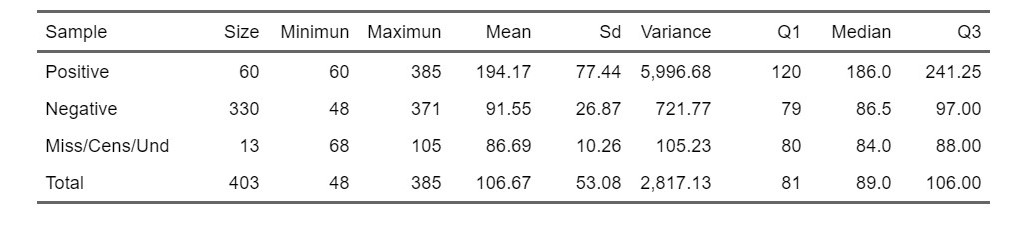
\includegraphics[width=14.0cm , height=3.25cm]{figures/TableStabGlu.jpeg} \\
\end{center}
\end{table} 

Left panel of Figure \ref{FE1} shows the kernel density estimations of the \textit{stabilized glucose} on positive and negative individuals generated through the code:
\begin{verbatim}
> library(ggplot2)
> density <- explore_plot(marker=diabet$stab.glu, status=diabet$diab)
> output  <- density$plot + xlab("Stabilized Glucose") +
                            scale_x_continuous(breaks = seq(0, 400, 50),
                                               labels = seq(0, 400, 50), 
                                               limits = c(0, 400))
> output
\end{verbatim}

\begin{figure}[h]
\begin{center}
\begin{tabular}{cc}
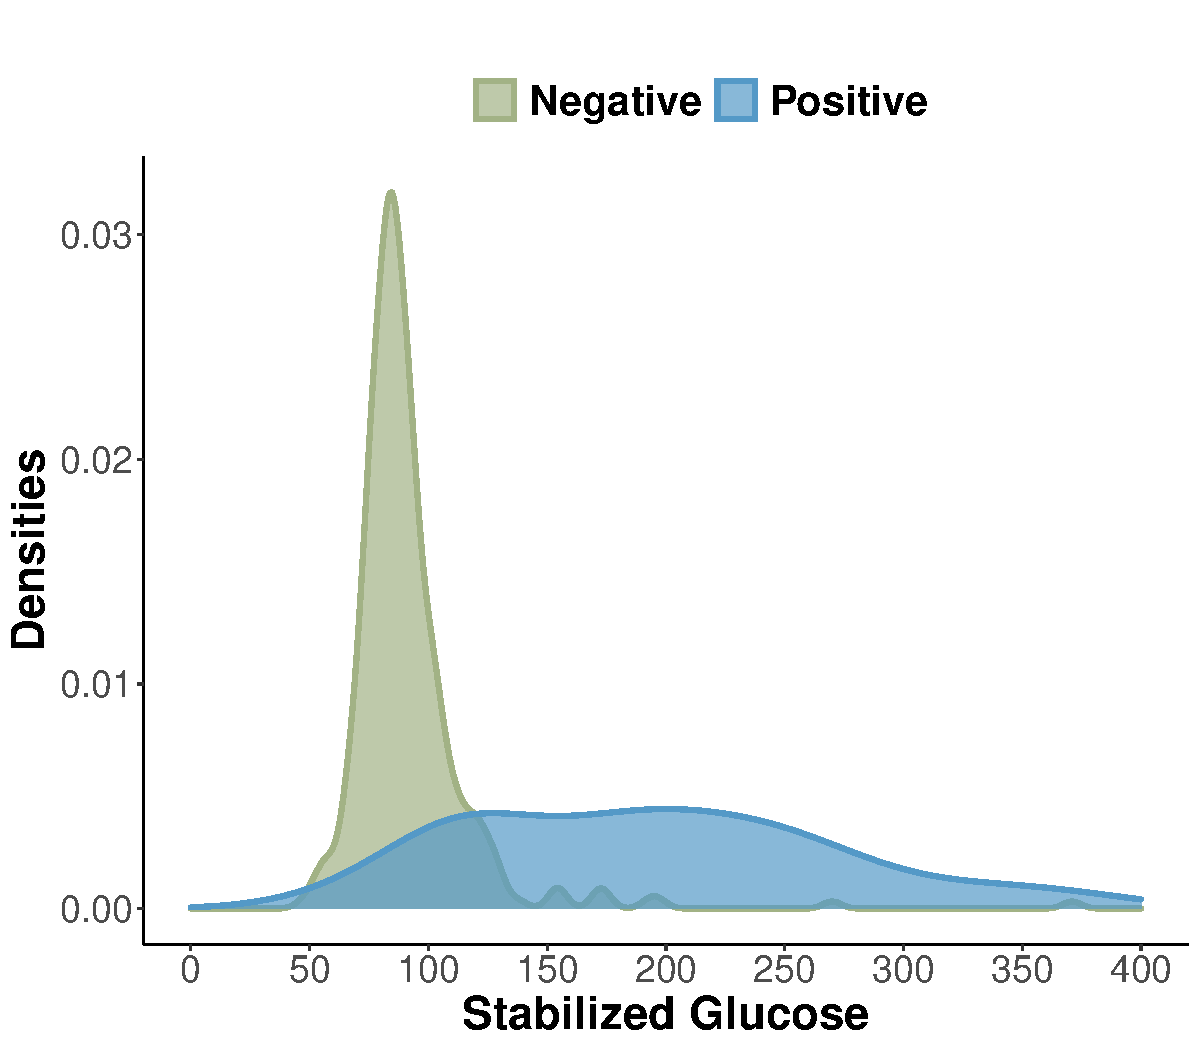
\includegraphics[width=7.0cm , height=6.75cm]{figures/FD1.pdf} & 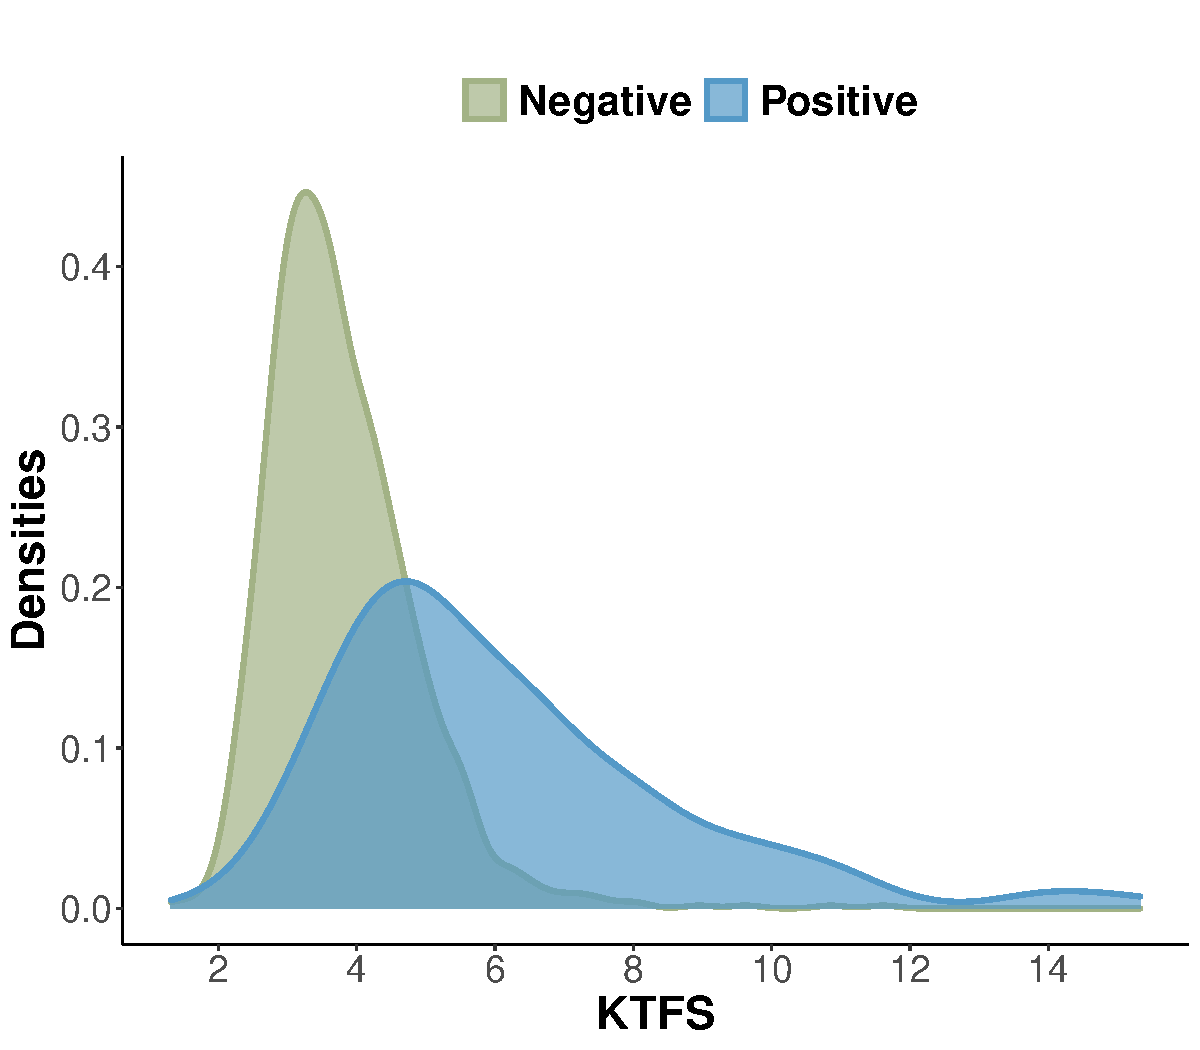
\includegraphics[width=7.0cm , height=6.75cm]{figures/FD2.pdf}
\end{tabular}
\caption{{\footnotesize{Left: Kernel density estimations of the {\textit{stabilized glucose}} biomarker on negative and positive individuals. Right: kernel density estimations of the {\textit{KTFS}} biomarker on negative and positive individuals after $5$ years from transplantation.} \label{FE1}}}
\end{center}
\end{figure} 

\subsection{Main function}
\textbf{sMSROC} is the main function in the package. It computes the sMS ROC curve estimator and its associated AUC with confidence intervals, estimated using the bootstrap percentile (BP) method, and according the approximations EVE and TVE given in Section 2. The function has the following input parameters:

\begin{itemize}
\item{\textbf{meth}} {method for approximating the predictive model ${\mathcal{P}}(D |x)$. There are several options available: 
\begin{itemize}
\renewcommand{\labelitemii}{-}
\item{\texttt{E}} {implements the naive method where missing, censored and undefined individuals are removed from the data.

}  
\item{\texttt{L}} {in the diagnosis scenario this option models the probability of being positive as: $${\mathcal{P}}(D | x) = \frac{1}{1 + \exp \{-(\beta_0 + \beta_1 \cdot x)\}},\quad \beta_0, \beta_1 \in \mathbb{R}.$$ 

In the case of prognosis scenarios under right censorship, a proportional hazards Cox regression model is used to approximate ${\mathcal{P}}(T \leq t | x)$ (and therefore, ${\mathcal{P}}(D | x)$). $${\mathcal{P}}(T \leq t | x) = 1 - \exp \{ -\Gamma_0(t) \cdot \exp \{ \beta \cdot x \}\},$$ where $\Gamma_0(\cdot)$ stands for the so-called cumulative baseline hazard function \citep{Cox1972}. Under interval censorship, ${\mathcal{P}}(T \leq t | x)$ is approximated through the model proposed in \citet{Diaz-Coto2020}:
 \begin{equation}
{\mathcal{P}} (T \leq t | x) =  \frac{S(U|x) - S(t|x) }{S(U|x) - S(V|x)}, \label{sdc1}
\end{equation}
where $U = \min{\{t, L\}}$ and $V = \max {\{t, R\}}$, being $L$ and $R$ the random variables depicting the edges of the observable interval $(L, R]$. 
The expression $S(t|x)$ stands for $S(t|X=x)$, that is, the survival function at $t$, given the marker value. 
It is estimated by proportional hazards model under interval censorship \citep{ Finkelstein1986}, applying linear interpolation inside the Turnbull intervals \citep{Turnbull1976}. 

In this case, the parameter {\bf{all}} indicates whether this approximation applied to all individuals or just to the mixed/censored/undefined ones.
}
\item{\texttt{S}} {approximates, in diagnosis scenarios, the logit transformation of the predictive model via a cubic spline function. That is: $${\mathcal{P}}(D | x) = \frac{1}{1 + \exp \{-s(x)\}},$$ where $s(\cdot)$ depicts some smooth function, estimated from restricted cubic splines \citep{Harrel2015}.
In the prognosis scenario under right censorship, we consider a proportional hazards model with a more flexible option to approximate the predictive model:
$${\mathcal{P}}(T \leq t | x) = 1 - \exp \{ -\Gamma_0(t) \cdot \exp \{ s(x) \}\},$$ where a penalized splines procedure \citep{Hurvich1998} estimates the smooth function $s(\cdot)$. Under interval censorship the predictive model is obtained by
$${\mathcal{P}} (T \leq t | x) = 1 - S(t|x),$$
where $S(t|x)$ is estimated as before through a proportional hazards model under interval censorship.
}
\end{itemize}
\item{\textbf{probs}} {a vector of manually entered predicted probabilities. This argument is useful if the user wants to estimate the predicted probabilities via a different model than the ones currently offered by the package. In this case, the argument {\textbf{meth}} will be ignored.}

\item{\textbf{sd.probs}} {a vector with the standard deviation of the probabilities entered as {\textbf{probs}}. It is an optional parameter.}
\item{\textbf{grid}} {grid size for computing the ROC curve estimate. The default value is 1000. It is also used to compute the AUC.}
\item{\textbf{conf.int}} {argument with two possible values indicating whether confidence intervals for the AUC will be computed (\texttt{T}) or not  (\texttt{F}).}
\item{\textbf{ci.cl}} {confidence level at which the confidence intervals for the AUC will be calculated. The default value is $95\%$.}
\item{\textbf{ci.meth}} {method for computing the AUC confidence intervals. There are three options available:
\begin{itemize}
\renewcommand{\labelitemii}{-}
\item{\texttt{V}} {method that uses the TVE variance approximation.}
\item{\texttt{E}} {method which uses the EVE approximation.}
\item{\texttt{B}} {confidence intervals based on BP.}
\end{itemize}}
} 
\item{\textbf{ci.nboost}} {number of bootstrap samples to be run when the option \texttt{B} is chosen as {\textbf{ci.meth}} parameter. The default value is 500.}
\item{\textbf{parallel}} {argument with two possible values which indicates whether parallel computing will be carried out (\texttt{T}) or not (\texttt{F}). There are two processes that currently support parallel computing: the \texttt{B} and \texttt{V} options to obtain confidence intervals for the AUC.}
\item{\textbf{ncpus}} {number of CPUS that will be used when parallel computing is chosen.}
\item{\textbf{all}} {parameter indicating whether all probabilities given by the predictive model should be considered (\texttt{T}) or only those corresponding to individuals whose condition as positive or negative is unknown (\texttt{F}).}
\end{itemize}

The sMSROC function returns an object of class {\textbf{sMSROC}}. It is a list of the following elements:

\begin{itemize}
\item{\textbf{thres}} {a vector of thresholds at which the sensitivity and the specificity have been computed.}
\item{\textbf{SE}} {a vector with the sensitivities at the considered thresholds {\textbf{thres}}.}
\item{\textbf{SP}} {a vector with the specificities calculated at the thresholds {\textbf{thres}}.}
\item{\textbf{probs}} {a vector with the predictive model estimates for each threshold. Recall that they represent the probability for the observations of being positive, given their marker values.}
\item{\textbf{u}} {sequence of points at which the sMS estimator will be computed. Its length is determined by the {\textbf{grid}} selection parameter.}
\item{\textbf{ROC}} {sMS ROC curve estimate computed at each value of the sequence {\textbf{u}}.}
\item{\textbf{time}} {the point of time at which the ROC curve has been computed, in the case of time-dependent outcomes.}
\item{\textbf{auc}} {area under the sMS ROC curve estimate. It is computed as the sum of the area of the rectangles whose base lies on two consecutive values of the sequence {\textbf{u}} and whose height is the sMS estimate value that corresponds to the lower edge of the base.}
\item{\textbf{auc.ci.cl}} {confidence level at which the confidence interval for the AUC has been computed.}
\item{\textbf{auc.ci.l}} {lower bound of the confidence interval for the AUC.}
\item{\textbf{auc.ci.u}} {upper bound of the confidence interval for the AUC.}
\item{\textbf{ci.meth}} {method used for estimating the confidence intervals for the AUC.}
\item{\textbf{data}} {a list whose elements are, in addition to the type of outcome handled, the set of parameters that had been used to compute the sMS estimator. The values for the {\textbf{grid}}, {\textbf{meth}}, {\textbf{parallel}} and {\textbf{ncpus}} elements are the default or those entered by the users. The {\textbf{marker}}, {\textbf{status}}, {\textbf{observed time}}, {\textbf{left}} and {\textbf{right}} vectors do not contain the positions that correspond to the missing marker values. The {\textbf{outcome}} element is a vector taking the value $1$ for the positive individuals; $0$, for negative and $-1$ for the missing/censored/undefined ones.}
\item{\textbf{message}} {a table with the warning messages generated along the computation process.}
\end{itemize}

The computation of the sMS ROC curve estimator is wrapped in three secondary functions according to each scenario. They have the same structure: a part in which the predictive model is estimated (first stage of the sMS estimator), 
and a common part where the remainder unknown elements are approximated through their empirical estimators (second stage of the sMS estimator).

The functions computing the predictive models have a common output: a list with the ordered marker values and their corresponding estimated probabilities. These two components and the {\textbf{grid}} are the input parameters of the \url{compute_ROC} function, which implements the computation of the second stage of the sMS estimator. This function provides: the sMS estimates for the sensitivity and the specificity according to the expressions given in (\ref{R23}) and (\ref{R24}); the ROC curve approximation obtained from these estimates (at the granularity level chosen through the {\textbf{grid}} parameter) and the underlying AUC. It is possible as well to directly enter the probabilities corresponding to the predictive model as parameter {\textbf{probs}}. In this case, none of the functions that compute the predictive model are called.

When the {\textbf{conf.int}} parameter is set to {\texttt {T}}, confidence intervals for the AUC are provided at the confidence level indicated as {\textbf{ci.cl}} parameter. They are computed according to the method entered as {\textbf{ci.meth}} parameter. 

\begin{itemize}
\item{When the chosen method is {\texttt {B}} the function \url{auc_ci_boot} is called and the confidence intervals based on BP are calculated. Depending on the type of outcome handled, the corresponding functions for computing the AUC under the sMS estimator are called {\bf ci.nboost} times. Since the bootstrap processes can be time-consuming, the function can be run in parallel via the argument {\textbf{parallel}}. In this case, the number of desired CPUs to be used should be indicated through the parameter {\textbf{ncpus}}. The package \CRANpkg{foreach} was used to implement the parallel computation.}
\item{Placing the option {\texttt {V}} as {\bf ci.method}, the function \url{auc_ci_nvar} is called and the confidence intervals are computed according to the asymptotic normality of the AUC estimator, based on the TVE approximation. The expression for the variance in this method depends on the variance of the predictive model estimates. That variance is calculated in an independent auxiliary function by bootstrapping (it is possible as well to perform parallel computation to carry out this task). When the probabilities of the predictive model have been directly entered by the users, there is also the option of indicating, manually, the corresponding standard deviation for these probabilities.}
\item{When the selected method is {\texttt{E}}, the function \url{auc_ci_emp} uses the asymptotic normality of the AUC estimator, in this case, the variance is calculated through the EVE approximation.}
\end{itemize}
The three functions have the same output: a list with two components, the lower and upper edges of the computed confidence intervals for the AUC.

\subsubsection{Example $1$ [ROC curve models]: the diabetes dataset}
Coming back to the diabetes dataset, we compute the ROC curves to assess the ability of {\textit{Stabilized glucose}} to identify patients with diabetes.  First, we only include this biomarker in the model, and since we observed that its distribution within the positive and the negative populations differs in location, spread, and shape, we used a smooth logistic regression for the first-stage estimation.
\begin{verbatim}
> roc_diabetes <- sMSROC(marker=diabet$stab.glu, status=diabet$diab,  meth="S")
> roc_diabetes

The AUC is 0.926. 
Predictive model computed through a smooth logistic regression model, based on 60 positive, 
330 negative, and 13 undefined (mixed) subjects.
\end{verbatim}

 The object \url{roc_diabetes} also contains the following components
\begin{verbatim}
> summary(roc_diabetes)

        Length Class  Mode     
thres    403   -none- numeric  
SE       403   -none- numeric  
SP       403   -none- numeric  
probs    403   -none- numeric  
u       1001   -none- numeric  
ROC     1001   -none- numeric  
auc        1   -none- numeric  
ci.meth    3   -none- character
data       6   -none- list     
message    4   -none- character
\end{verbatim}
which allow to perform a number of customized figures and analyses, including the selection of thresholds under different criteria.

On the other hand, if we want to use an alternative model in the first-stage, for instance, by including additional information which could help us to have a more accurate prediction of the real status of the undefined subjects, we just have to perform this first-stage out of the sMSROC function, and save the vector of the predicted probabilities. This is illustrated in the following chunk of code, where we use logistic regression with first-order effects for both the biomarker and age.
\begin{verbatim}
> alt_mod <- glm(diab ~ diabet$stab.glu + diabet$age, family = 'binomial')
> prob_model <- predict(alt_mod, type = 'response',
                        newdata = data.frame(diabet$diab, diabet$stab.glu, diabet$age))
\end{verbatim}
Then, we include these probabilities in the function
\begin{verbatim}
> roc_diabetes_prob <- sMSROC(marker=diabet$stab.glu, status=diabet$diab, 
                              probs=prob_model)
> roc_diabetes_prob

The AUC is 0.886.
Predictive model externally computed. Based on 0 positive, 0 negative, 
and 403 undefined (mixed) subjects.
\end{verbatim}

Notice that, in this example, all the subjects are considered as mixed, since none of them are considered as fully positive not fully negative. If we would want to apply this model only on those subjects for which the actual status is unknown, we should introduce probabilities of $1$ of $0$ for the actually positive, and actually negative, respectively.


\subsubsection{Example $2$ [ROC curve models]: the kidney transplant failure score (KTFS) dataset}
In this second example, our aim is to evaluate the prognostic ability of the {\textit{Kidney Transplant Failure Score}} (KTFS) to predict the graft failure after five years from kidney transplantation. The KTFS is a composite score build on the base of accepted risk factors of graft loss \citep{Foucher2010}. We will use a subset of the DIVAT cohort (\url{https://www.divat.fr}) delivered at the \CRANpkg{RISCA} package, and now also included in our package. This dataset, {\bf{ktfs}}, contains the follow-up time from transplantation in years to either of the graft failure or the censoring time (in many cases due to death), a graft failure indicator, and the KTFS score for 2,169 kidney transplant recipients. The distribution of the KTFS score on both patients with graft failure within 5 years (108), and those with a functional graft after 5 years (954) was depicted in Figure \ref{FE1} (right). Notice that 1107 patients were undefined (follow-up below 5 years and graft working).

\begin{verbatim}
> data(ktfs)
> roc_KTFS <-  sMSROC(marker=ktfs$score, status=ktfs$failure,
>              observed.time=ktfs$time, time=5, meth="L",
>              conf.int="T", ci.meth ="E")  

The AUC is 0.763. 
Predictive model computed through a Cox PH regression model, based on 108 positive, 954 negative, 
and 1107 undefined (mixed) subjects.
\end{verbatim}

\subsection{Summarize and plot functions}
The \CRANpkg{sMSROC} package includes functions which provide numerical and graphical summaries of the data contained in the object returned by the {\textit{sMSROC}} function. We describe them below.  

The \url{sMSROC\_plot} provides informative plots of the sMS ROC curve estimate. The function has the following input parameters:

\begin{itemize}
\item{\textbf{sMS}} {an object of class {\textbf{sMSROC}}.} 
\item{\textbf{m.value}} {marker value. When specified, the point which corresponds to that marker value is added over the plot of the ROC curve.}
\end{itemize}

The function generates two different types of graphics. On one hand, it computes a basic plot approximating the ROC curve by the pairs given by the sequences {\textbf{1 - SP}} and {\textbf{SE}}, from the {\textbf{sMSROC}} object. We have added to this plot the layers {\texttt{geom\_roc()}} and {\texttt{roc\_style()}} from the  \CRANpkg{plotROC}  package, to obtain a final object that could take advantage of the whole functionality of this package. On the other hand, we produce a customized graphic of the ROC curve whose class is {\textbf{ggplot}} by plotting the sequence {\textbf{1 - SP}} against {\textbf{SE}}. In the case that a number of {\textbf{m.value}} is indicated, the final plot displays over the ROC curve line the point that corresponds to the entered value.

The output of the function is a list with two components:
\begin{itemize}
\item{\textbf{basic.plot}} {an object that can be used and customized using the tools from the  \CRANpkg{plotROC} package.} 
\item{\textbf{roc.plot}} {an object of class {\textbf{ggplot}}. Although it is already customized (e.g. title, colors or axis labels) the users can make their own changes by adding the corresponding layers through the tools available in the \CRANpkg{ggplot2}  package.}
\end{itemize}
The function {\url{evol\_AUC}} provides a graphic with the areas under the time-dependent ROC curves computed by the sMS estimator over a sequence of times. Its input parameters include the sample information for time-dependent outcomes ({\textbf{marker}}, {\textbf{status}}, {\textbf{observed.time}}, {\textbf{left}} and {\textbf{right}}); the {\textbf{time}}, that in this case is a vector containing the points of time at which the AUC will be computed; the method of computation ({\textbf{meth}}) and the {\textbf{grid}}. The features of these parameters are the same  described for the corresponding functions in the package. The function \url {evol\_AUC} calls \url{sMSROC} at each of the times indicated in the vector {\textbf{time}}, and the AUC is computed according to the parameters indicated. The output is a list with three elements:
\begin{itemize}
\item{\textbf{evol.auc}} {an object of class {\textbf{ggplot}}. It is a graphic line plotting the AUCs at the considered times.} 
\item{\textbf{time}} {a vector with the values of the {\textbf{time}} entered as parameter.}
\item{\textbf{auc}} {a vector with the values of the AUCs computed at the times indicated at the {\textbf{time}} parameter.}
\end{itemize}
The function \url{pred\_probs} plots the predicted probabilities estimated from the predictive model for each of the marker values. It may provide a $95\%$ pointwise confidence intervals. The input parameters of the function are:
\begin{itemize}
\item{\textbf{sMS}} {an object of class {\textbf{sMSROC}}.} 
\item{\textbf{var}} {argument with two possible values indicating whether the pointwise confidence intervals should be computed (\texttt{T}) or not (\texttt{F}).}
\item{\textbf{nboost}} {number of bootstrap samples for computing the pointwise confidence interval.}
\item{\textbf{parallel}} {argument indicating whether parallel computing will be carried out (\texttt{T}) or not (\texttt{F}).}
\item{\textbf{ncpus}} {number of CPUS to be used in the case of choosing parallel computing.}
\end{itemize}
The function \url{pred\_probs} generates a graphic for the probability estimation of the predictive model versus the marker values. As usual, this is a {\textbf{ggplot}} object which can be customized by the user. In the case that the {\textbf{var}} option is set to \texttt{T}, the function computes and plots $95\%$ pointwise confidence intervals on the same graphic. The variance of the probability estimates is computed via bootstrap. The output of the function is a list with four components:
\begin{itemize}
\item{\textbf{plot}} {an object of class {\textbf{ggplot}}.} 
\item{\textbf{thres}} {a vector of marker values (x-axis coordinates).}
\item{\textbf{probs}} {a vector containing the predicted probabilities (y-axis coordinates).}
\item{\textbf{sd.probs}} {a vector containing the estimation of the deviation of the predicted probabilities.}
\end{itemize}
\subsubsection{Example $2$ [ROC curve plots]: the kidney transplant failure score (KTFS) dataset}
The next piece of code returns the plot of the ROC curve computed on the data from the {\textit{KTFS}} example (top-left). We only show the basic plot, however, it can be customized with elements from the \CRANpkg{plotROC} package. The code also generates the probabilities derived from the predicitive model used in the first stage (i.e. proportional hazard Cox regression), and included in the same panel (top-right), and the evolution of the AUC over ten years from kidney transplantation (bottom).

\begin{verbatim}
> # ROC curve
> plot_KTFS <- sMSROC_plot(sMS = roc_KTFS, m.value = 3.9)
> plot_KTFS$rocplot
>
> # Evolution of the AUCs
> aucs <- evol_auc(marker = ktfs$score, status = ktfs$failure,
>                  observed.time = ktfs$time,
>                  time = seq(2, 10), meth = "L")
> plot_aucs <- aucs$evol.auc +
>              scale_x_continuous(limit = c(2, 10),
>                                 breaks = seq(2, 10, 1)) +
>              scale_y_continuous(limit = c(0.4, 1),
>                                 breaks = seq(0.4, 1, 0.1))
> df1 <- data.frame(x = c(2,10), y = c(0.5, 0.5))
> plot_aucs <- plot_aucs +
> geom_line(data = df1, aes(x, y), linewidth = 0.9, colour = "gray", linetype = "twodash")
> plot_aucs
>
> # Predictive model
> probs <- probs_pred(roc_KTFS, var = "T")
> plot_probs_pred <- probs$plot + xlab("KTFS")
> plot_probs_pred
\end{verbatim}

All these plots are arranged in the Figure \ref{FE2}.\par
\vspace{0.5cm}\noindent
\begin{figure}[h]
\begin{center}
\begin{tabular}{c}
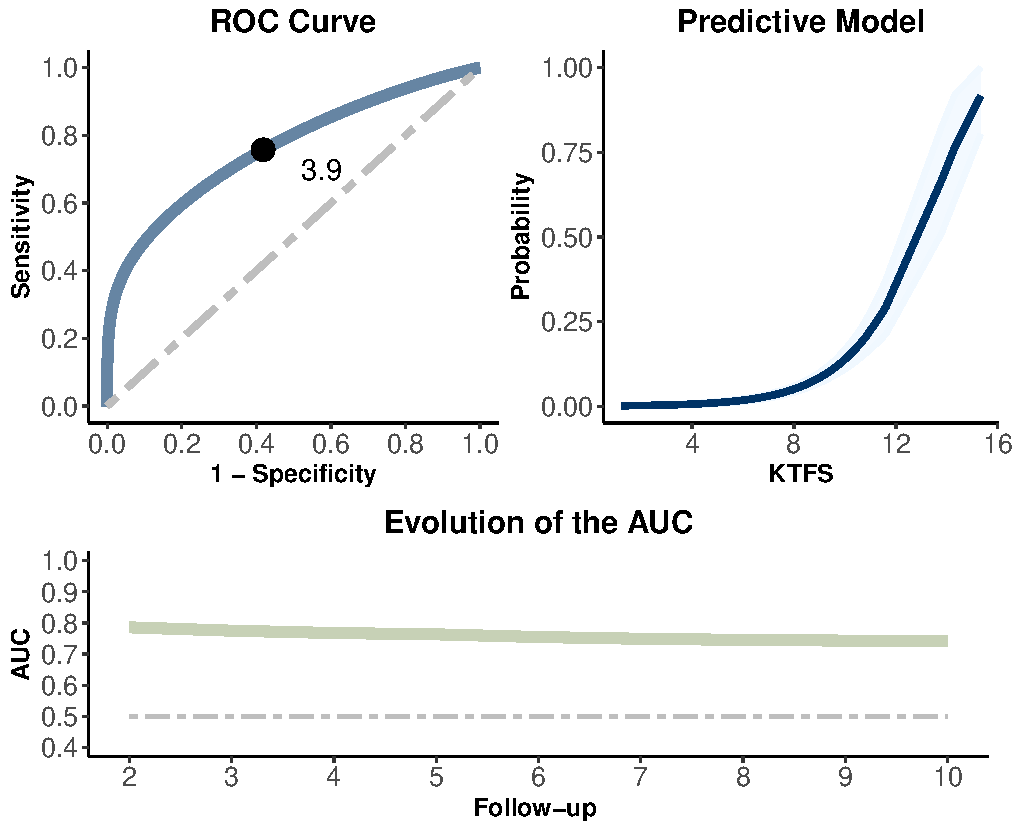
\includegraphics[width=12.0cm]{figures/FE2.pdf} 
\end{tabular}
\caption{{\footnotesize{Upper left: graphic of ROC curve estimate obtained from the \url{sMSROC_plot} function, customized to show the point of the curve corresponding to a given {\it{KTFS}} value. Upper right: estimated probabilities from the predictive model with $95\%$ pointwise confidence intervals computed for the biomarker. Bottom: evolution of the  AUCs over 10 years from kidney transplantation for the {\it{KTFS}} score.} \label{FE2}}}
\end{center}
\end{figure} 

Finally, the function {\url{conf\_int\_print}} prints the values, method of computation, and the confidence level of the confidence intervals calculated for the AUC. Since the {\textbf{sMSROC}} object may contain information stored in large list of components, we only print a single summary, such as the lower and the upper bounds of the confidence intervals, the level at which they were obtained, and the method used for their computation. The input of this function is an object of class {\textbf{sMSROC}} and the output is a string including the described information. As example, below is shown the code for printing the AUC and $95\%$ confidence intervals for the {\textit{KTFS}} at $5$ years:

\begin{verbatim}
> conf.int.print(roc_KTFS)
"AUC: 0.76; 0.95\% C.I.[0.6, 0.93]"
\end{verbatim}

\section{Example 3: the fibrosis dataset}
We finally consider the fibrosis dataset. This synthetic data set ships alongside singR and emulates a retrospective study carried out at three different medical centers in Spain. The goal was to determine the 
capacity of a score punctuation (based on the age, different polymorphisms, and other variables) to predict the worsening of the fibrosis stage in patients with chronic Hepatitis C (HC). A total of 
722 individuals infected by the HC virus, and underwent revision since a particular date were enrolled. The date of the diagnosis of HC and a number of variables determining the risk score such as the age, gender, alcohol consumption, and different polymorphism variants were also collected. Reader interested in having more information about the original study are referred to \citet{JoseRamon2020}.

Particularly, we are interested in knowing the prediction ability of the constructed risk score at 5, 10, and 15 years from the HC onset. However, for each patient, we only know whether or not  the fibrosis worsened within the interval $(0,R_i]$ or $(R_i, \infty)$ ($1\leq i\leq 722$), where $R_i$ is the time between the diagnosis and the revision dates. Therefore, we have an interval censorship scenario in which, for instance, at 5 years, the $i$th patient is positive if they were positive in the revision and $R_i\leq 5$, negative if they was negative in the revision and $R_i\geq 5$, and undefined otherwise. The next piece of code deals with the ROC curve construction at 5 years. Since higher values of the score are associated with smaller probabilities of having the event, we have transformed the values adequately.

\begin{verbatim}
> data(fibrosis)
> explore_table(marker = -fibrosis$Score, left = fibrosis$Start,
>                 right = fibrosis$Stop, time = 5)$summary
\end{verbatim}

\begin{verbatim}
         Sample Size Minimun Maximun   Mean   Sd Variance  Q1 Median Q3
1      Positive   21      -8      -2  -5.95 1.63     2.65  -7     -6 -5
2      Negative  112     -22      -3 -11.30 3.21    10.30 -13    -11 -9
3 Miss/Cens/Und  589     -21      -3 -10.02 3.09     9.56 -12    -10 -8
4         Total  722     -22      -2 -10.10 3.19    10.19 -12    -10 -8
\end{verbatim}


\begin{verbatim}
> roc_fibrosis_5 <- sMSROC(marker = -fibrosis$Score, left = fibrosis$Start, 
>                        right = fibrosis$Stop, meth = "L", time = 5)
> roc_fibrosis_5

The AUC is 0.647. 
Predictive model computed through a D. Finkelstein PH regression model, accounting to 
the length of the observed intervals, based on 21 positive, 112 negative 
and 589 undefined (mixed) subjects.

> sMSROC_plot(roc_fibrosis_5)$rocplot
\end{verbatim}

Figure \ref{FE3} shows the ROC curves at 5, 10, and 15 years using the sMS ROC curve estimates (top-left), and the estimator proposed by \citet{Kassu2022} (top-right) and recently implemented in the package \CRANpkg{cenROC}. Besides, since the object \url{roc_fibrosis_5} also contains the values of both the sensitivity and 
the specificity for each potential threshold, the next simple piece of code allows to compute the weighted Youden index \citep{Pablo2011}. $$J_{\lambda}=\max_{x\in\mathbb R}\{\lambda\cdot Se(x)+ (1-\lambda)\cdot Sp(x)\}\quad \lambda\in [0,1],$$ and its associated threshold. Figure \ref{FE3} (middle) depicts $J_\lambda$ at 5 years, and highlights some of the thresholds. Notice that $J_{1/2}$ is equivalent to the Youden index. We also include the AUC evolution along the follow-up computed through the \CRANpkg{sMSROC} (blue line) and \CRANpkg{cenROC} (red line) packages. AUCs at 5, 10, and 15 years were 0.647, 0.680 and 0.687 for the sMS ROC curve (Figure \ref{FE3} bottom), and 0.640, 0.653 and 0.680 for the cenROC-based estimations.  

\begin{verbatim}
> lambda <- seq(0, 1, length = 101)
> Yw <- seq(0, 1, length = 101)
> Tw <- seq(0, 1 ,length = 101)

> for (j in 1:101) {
> Yw[j]<- max(lambda[j]*roc_fibrosis_5$SE + (1-lambda[j])*roc_fibrosis_5$SP)
> Tw[j]<- roc_fibrosis_5$thres[which.max(lambda[j]*roc_fibrosis_5$SE + 
                                        (1-lambda[j])*roc_fibrosis_5$SP)]}
\end{verbatim}

\vspace{0.5cm}\noindent
\begin{figure}[h]
\begin{center}
\begin{tabular}{c}
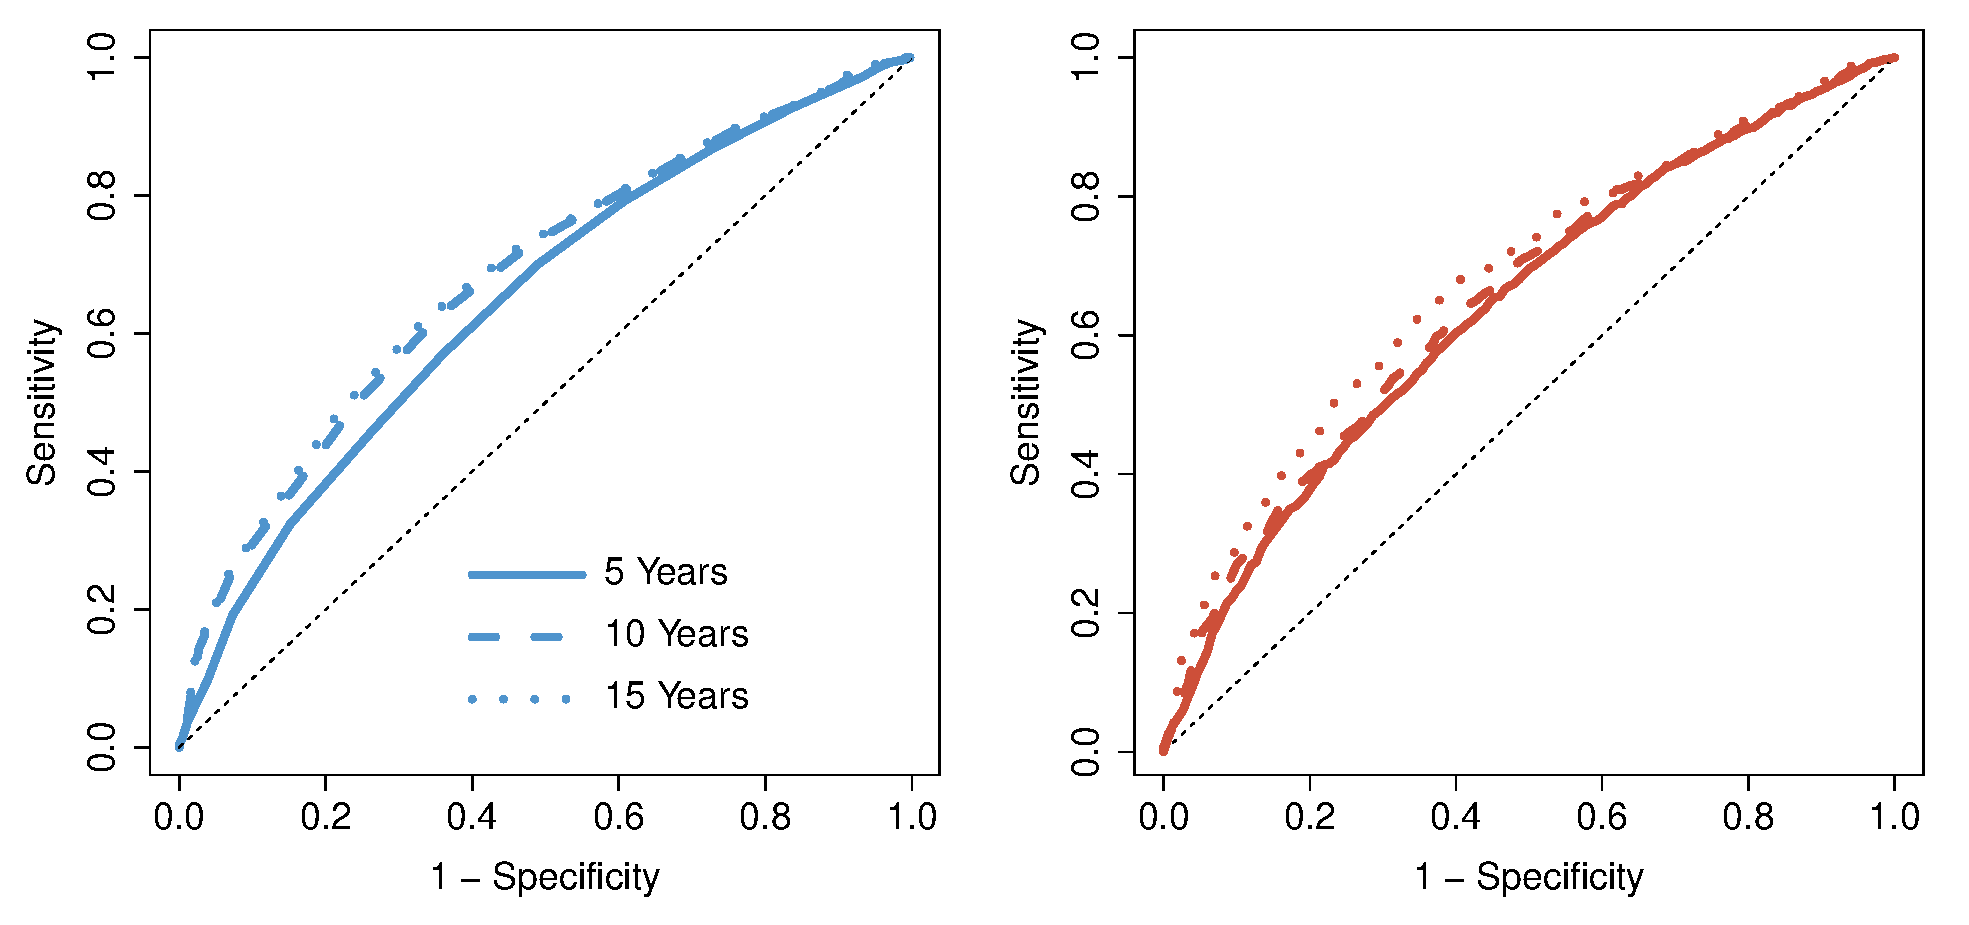
\includegraphics[width=12.0cm]{figures/ROCFigure3.pdf} \\
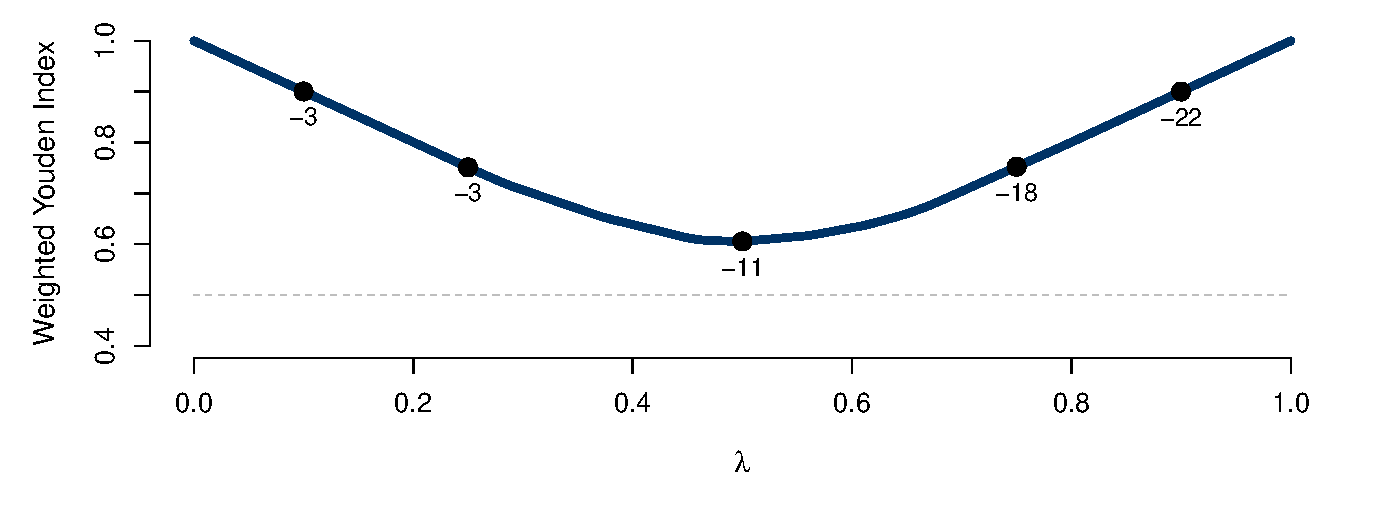
\includegraphics[width=12.0cm]{figures/YoudenFigure3.pdf} \\
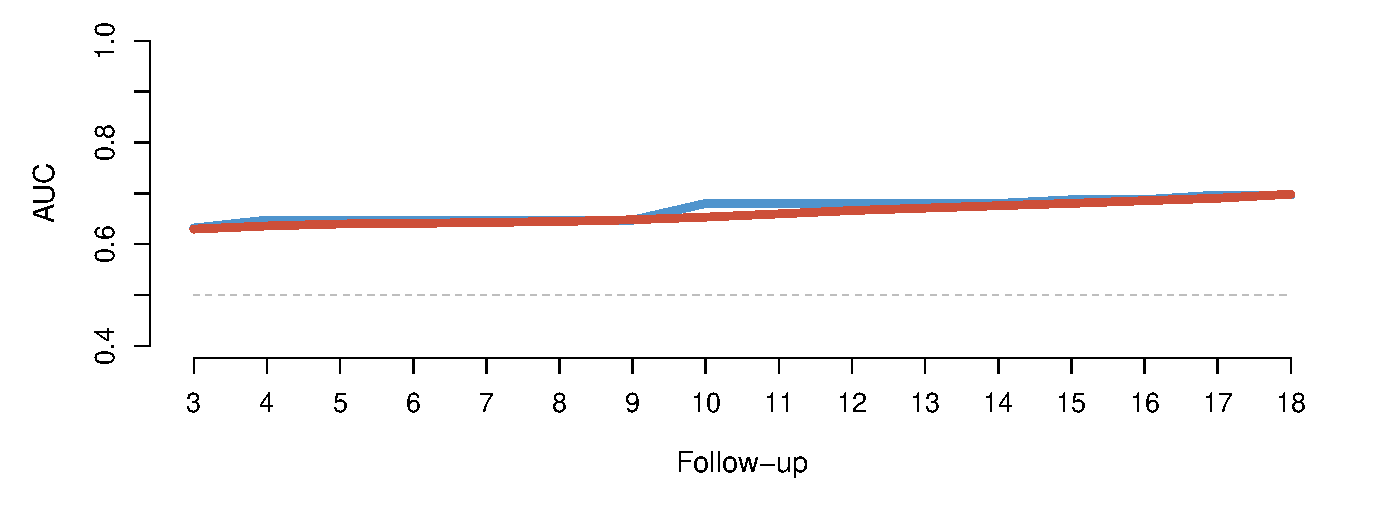
\includegraphics[width=12.0cm]{figures/AUCFigure3.pdf} \\
\end{tabular}
\caption{{\footnotesize{Top: ROC curves estimates at 5, 10 and 15 years from the \CRANpkg{sMSROC} (left), and from the \CRANpkg{cenROC} (right) packages. Middle: Weighted Youden Index at 5 years from the sMS ROC curve estimation. Bottom: AUC evolution from 3 to 18 years for the two considered estimators}. \label{FE3}}}
\end{center}
\end{figure} 

\section{Conclusions}
We presented the new \url{R} package \CRANpkg{sMSROC} which implements the two-stage mixed-subjects ROC curve estimator. This procedure allows the user to assess the classification performance of both diagnostic and prognostic biomarkers. The package offers a set of exploratory functions which allow researches to have an insight of the distribution of the biomarkers on positive and negative individuals, and on those whose status is unknown. 
A single main function ({\url{sMSROC}}) wraps secondary functions developed to compute the sMS estimator, and the AUC with a confidence interval.
This method allows to link the diagnosis and prognosis scenarios via a predictive model which models the relationship between the biomarker and the event under study. The most common probabilistic models (e.g. logistic regression, Cox proportional hazards regression) are implemented out-of-the-box and the user can also enter their own predicted probabilities which can be computed using any other appropriate model. A separate function computes the weighted empirical estimator of the biomarker to get the corresponding estimates for the sensitivity and specificity (second stage). 
We also implemented three different ways of computing the variance of the AUC and these are available in the package. The package also contains several summarize functions which provide useful numerical and graphical outputs. These include the ROC curve plots, a plot of the evolution of the AUC over time, or the plots of the predictive models. 

\section*{Appendix}
Assume a sample with $N$ subjects. Let $\{\hat {\cal P}(D|x_1),\cdots , \hat {\cal P}(D|x_N)\}$ be the individual estimated probabilities of being within the positive group, and let $\{ \hat\sigma^2(x_1), \cdots , \hat\sigma^2(x_N)\}$ be their respective variance. 
Then, if $\hat\pi_N= N^{-1}\sum_{i=1}^N \hat {\cal P}(D|x_i)$, the TVE approximation for the variance of AUC is
\begin{equation*}
\text{TVE}= \frac{1}{[\hat\pi_N\cdot (1 - \hat\pi_N])^2}\cdot [\hat v_1^2 + \hat v_2^2],
\end{equation*}
where
\begin{align*}
\hat v_1^2=& N^{-1}\sum_{j=1}^N \left\{ [\hat W_{\text{se}}(x_j) + \hat W_{\text{sp}}(x_j)]\cdot {\cal P}(D|x_j) - \hat W_{\text{sp}}(x_j)\right\}^2, \quad\text{ and} \\
\hat v_2^2=& \left\{ N^{-1}\cdot \sum_{j=1}^N [\hat W_{\text{sp}}(x_j) - \hat W_{\text{se}}(x_j)]\dot\hat\sigma_(x_j)\right\}^2,
\end{align*}
and with
\begin{align*}
\hat W_{\text{se}}(x)=& N^{-1}\sum_{j=1}^N[I_{(x_j,\infty)}(x) - \widehat {\text Se}(x_j)]\cdot [ 1 - \hat {\cal P}(D|x_j)],  \quad\text{ and} \\
\hat W_{\text{sp}}(x)=& N^{-1}\sum_{j=1}^N[I_{(x_j,\infty)}(x) - \widehat {\text Sp}(x_j)]\cdot \hat {\cal P}(D|x_j),
\end{align*}
$I_A(s)$ is the indicator function (takes the value $1$ if $s\in A$, and $0$ otherwise) and $\widehat {\text Se}(\cdot)$ and $\widehat {\text Sp}(\cdot)$ are the estimates for the sensitivity and the specificity, respectively. The most challenging part of approximating the variance is usually the computation of $\hat\sigma^2(\cdot)$. When $\hat {\cal P}(D|x)$ is based on logistic or Cox-type regression models, closed-form equations for estimating the variance are available. However, these equations are 
based on the Delta-method and the obtained results are sometimes not good estimates. The EVE approximation considers that the proposed AUC estimator variance is similar to the one based on the empirical estimator of the observed subjects, and therefore it could be approximated through
\begin{equation*}
\text{EVE}= \frac{N}{N_O}\cdot \left\{ \frac{1}{1-\hat\pi_N}\cdot <\widehat {\text{Se}}, \widehat {\text {Sp}}> + \frac{1}{\hat\pi_N}\cdot <\widehat {\text{Sp}}, \widehat {\text {Se}}>\right\},
\end{equation*}
where given two real functions $f$ and $g$, $<f,g>=\int f^2dg - (\int fdg)^2$, and $N_O$ is the number of subjects with complete information (those used for estimating the predictive model).


\bibliography{SusanaDiazCoto}

\address{Susana D\'iaz-Coto\\
Department of Orthopaedics, Dartmouth Health, Lebanon, NH, USA \\
Geisel School of Medicine at Dartmouth, Hanover, NH, USA\\}
\email{Susana.Diaz.Coto@Hitchcock.org}

\address{Pablo Mart\'inez-Camblor\\
Faculty of Health Sciences, Universidad Autonoma de Chile, Chile\\
and \\
Department of Anesthesiology, Dartmouth Health, Lebanon, NH, USA \\
Geisel School of Medicine at Dartmouth, Hanover, NH,  USA\\}
\email{Pablo.Martinez-Camblor@Hicthcock.org}

\address{Norberto Corral-Blanco\\
Department of Statistics, Operational Research and Mathematics Didactics, University of Oviedo, Oviedo (Asturias), Spain\\}
\email{norbert@uniovi.es}


























